\section{Probing radiation}

This work is focussed on the use of X-ray and neutron scattering, therefore it is pertinent to discuss how each of these probing radiation is produced and detail the advantages of each with resepect to the other.

\subsection{The generation of X-ray and neutrons}

\subsubsection{X-rays}

X-rays are a form of electromagnetic radiation similar to visible light, albeit with a much shorter wavelength -- from \SI{0.01}{\nano\meter} to \SI{10}{\nano\meter}. There are three common ways to produce X-rays; two are available within the laboratory, while the other is exclusive to large scale facilities.

The two laboratory source X-ray generation techniques are the X-ray tube and the rotating anode. An X-ray tube consists of a filament and an anode within a vacuum chamber, by passing a high voltage electrical current across the filament electrons are emitted which accelerate towards the anode. On collision with the anode, the rapid deceleration results in the emission of X-rays of a characteristic wavelength based on the anode material.\cite{Schnablegger2017} The most common material for an X-ray tube anode is copper which gives off radiation of about \SI{8}{\kilo\eV}.

The other common laboratory method for the generation of X-rays is the rotating anode, which is an improvment on the X-ray tube. In the X-ray tube, each time that an electron contacts the anode there is some energy transfer, this means that over many millions of collisions, the temperature of the anode can raise significantly -- leading to a temperature limitation on the X-ray flux available. This lead to the development of the rotating anode, this is simply where the anode is made from a rotating wheel, so that the bombardment is spread across the whole wheel reducing the energy localisation. This allows an increase in the photon flux by about an order of magnitude.\cite{Schnablegger2017}

The third method of X-ray generation is at a synchrotron facility, this method has the drawback that it requires access to a national or international faciliy; such as Diamond Light Source (DLS) or the European Synchrotron Radiation Facility (ESRF). The way in which X-rays are generated at the synchrotron involves the acceleration of an electron, rather than the deceleration as with the laboratory sources. This is achieved by having relativistic electrons travel in around a curve, from Newtonian mechanics it is known that travelling on a curve at constant speed is equivalent to acceleration. This is achieved by firstly accelerating the electrons, produced in an linear accelerator (Linac), to near the speed of light in a booster synchrotron before injecting them into the storage ring. In the storage ring, the electrons are kept at relativistic speeds with bending magnets (BM) and straight sections making up a ring (Figure \ref{fig:syn}). The circularity of the ring is dependent on the number of bending magnets that make up the ring; for example, DLS has 48 bending magnets with 48 straight sections.
%
\begin{figure}
	\centering
	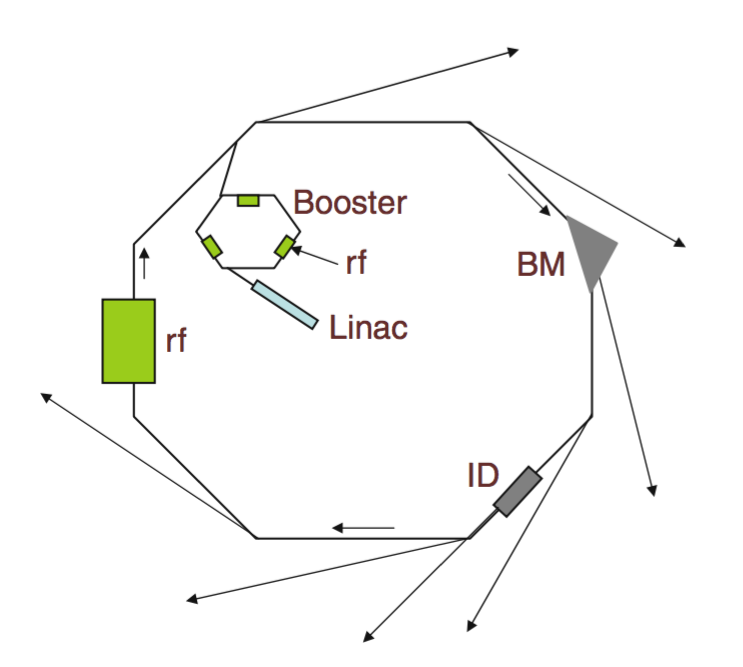
\includegraphics[width=0.7\textwidth]{theory/syn}
	\caption{A schematic representation of a synchrotron radiation source, identifying the Linac, the booster ring, the radio-frequency cavities (rf), the bending magnet (BM) and the insertion device (ID), from Ref \cite{Garcia-Gutierrez2009}.}
	\label{fig:syn}
\end{figure}
%

When an electron accelerates (or travels on a curve), Cherenkov radiation is emitted in accordance with the Cherenkov relation,
%
\begin{equation}
	n_i\beta_c\cos{\theta_e} = 1,
\end{equation}
%
where, $n_i$ is the refractive index for the dielectric medium, $\beta_c$ is the fraction of the speed of light at which that electron is travelling, and $\theta_e$ is the angle between the electron trajectory and the trajectory of the resulting photon.\cite{Garcia-Gutierrez2009} The curve is the result of a bending magnet, meaning that at each bending magnet there can be a beamline which gives out synchrotron light. The light this is given off from a bending magnet is continuous and broad, covering a wide range of the electromagnetic spectrum. The alternative to a bending magnet beamline is a beamline which is served by an insertion device (ID). An insertion device is able to offer more specific radiation characteristics (photon energy, narrower band) than a bending magnet, and are placed on the magnet-free straight sections of the synchrotron. Common insertion devices include wavelength shifters, wigglers, and undulators.

The type of insertion device that is present at both I07 and I22 at DLS is an undulator. An undulator consists of a series of magnets of opposing polarity whihc causes the electrons to `wiggle' back and forth (Figure \ref{fig:undulator}). This results in a superposition of radition from $N_P$ sources, where $N_P$ si the number of magnets, yielding quasi-monochromatic radiation. The brilliance of different X-ray sources are compared in Table \ref{tab:sources}, this shows the significant benefit that an undulator offers in terms of photon brilliance.
%
\begin{figure}
	\centering
	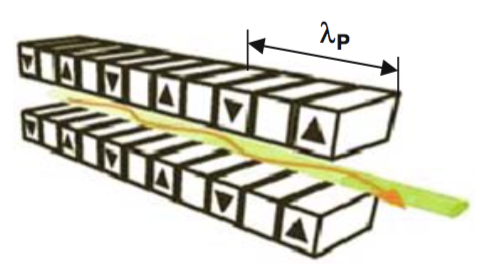
\includegraphics[width=0.7\textwidth]{theory/undulator}
	\caption{A diagram of an undulator insertion device such as that on I07 or I22 where $\lambda_P$ is the period length between opposing magnets, from Ref \cite{Garcia-Gutierrez2009}.}
	\label{fig:undulator}
\end{figure}
%
%
\begin{table}
	\centering
	\caption{A comparision of the photon brilliance from different light sources, adapted from Ref \cite{Sivia2011}.}
	\label{tab:sources}
	\begin{tabular}{l | c}
		\toprule
		\multirow{2}{*}{Light source } & Approximate brilliance/ \\
 & \si{\second^{-1}\milli\radian^{-2}{0.1}\percent bandwidth^{-1}} \\
		\midrule
		Candle & $10^5$ \\
		X-ray tube & $10^8$ \\
		Sun & $10^{10}$ \\
		Bending magnet & $10^{15}$ \\
		Undulator & $10^{20}$ \\
		\bottomrule
	\end{tabular}
\end{table}

\subsubsection{Neutrons}
